\documentclass[12pt]{article}
\usepackage[utf8]{inputenc}
\usepackage[T1]{fontenc}
\usepackage{lmodern}
\usepackage{setspace}
\usepackage{geometry}
\usepackage{url}
\usepackage{graphicx}

\geometry{
  left=1in,
  right=1in,
  top=1in,
  bottom=1in
}

\begin{document}

%-------------------------------
%           TITLE PAGE
%-------------------------------
\begin{titlepage}
\begin{center}

{\Large \textbf{ASL Recognition System:\\[6pt] Bridging Gaps in Communication Accessibility}}\\[2cm]

{\normalsize A Thesis Submitted in partial fulfillment of the Requirements of the\\
Renée Crown University Honors Program at Syracuse University}\\[1.5cm]

{\large \textbf{Carlo F. Pisacane}}\\[0.5cm]
{\normalsize Candidate for Bachelor’s of Science in Computer Science\\
and Renée Crown University Honors\\
May 2025}\\[3cm]

{\Large \textbf{Honors Thesis in Computer Science}}\\[1.5cm]
\begin{tabbing}
\hspace*{3cm}\= \kill
Thesis Advisor:\> \underline{\hspace{4cm}} \\
\> Dr.\ Nadeem Ghani, Assistant Teaching Professor\\[1cm]
Thesis Reader:\> \underline{\hspace{4cm}} \\
\> Dr.\ João Paulo Marum, Assistant Teaching Professor\\[1cm]
Honors Director:\> \underline{\hspace{4cm}} \\
\> Dr.\ Danielle Smith, Director
\end{tabbing}
\vfill

\end{center}
\end{titlepage}

\clearpage
\pagenumbering{roman}
\setcounter{page}{1}
\pagestyle{plain}


\newpage
\vspace*{\fill}        
\begin{center}
    {\small © Syracuse University 2025. All rights Reserved}
\end{center}
\vspace*{\fill}
\newpage

%-------------------------------
%           ABSTRACT
%-------------------------------
\clearpage
\section*{Abstract}
\vspace{1em}

\noindent
A concise summary of your research, covering the problem (gaps in existing ASL recognition 
systems), your proposed solution (ASL recognition tool), methodology, key findings, and
conclusions. 

\vspace{2em}
\noindent
\textbf{Thesis Advisor:} Nadeem Ghani \\
\textbf{Title:} Assistant Teaching Professor, Engineering and Computer Science

\newpage
\mbox{}                
\newpage

%-------------------------------
%       ACKNOWLEDGMENTS
%-------------------------------
\newpage
\doublespacing
\section*{Acknowledgments}

I am deeply grateful for the support and guidance I have received throughout my academic journey at Syracuse University. I would like to extend my sincere thanks to my advisor, Prof. Nadeem Ghani, whose mentorship was instrumental in shaping my research and academic pursuits. My gratitude also goes to my thesis reader, Prof. João Marum, for his valuable insights and constructive feedback.

I am particularly thankful to Robin Smith, my Honors advisor, for motivating and encouraging me over the past four years during my time in the Honors program and throughout the thesis development process. Their support helped me overcome challenges and remain focused on my goals.

Finally, I am forever indebted to my friends and family, whose encouragement and belief in me have been a constant source of inspiration.


%-------------------------------
%       Preface
%-------------------------------
\newpage
\doublespacing
\section*{Preface}

Why I chose this topic, personal insights, and what I learned, reference: CS example 
thesis.pdf (Kyle Maiorana)

\clearpage
\pagenumbering{arabic}
\setcounter{page}{1}
\doublespacing

%-------------------------------
%     TABLE OF CONTENTS
%-------------------------------
\newpage
\tableofcontents
\newpage

%-------------------------------
%   CHAPTER 1 / INTRODUCTION
%-------------------------------
\doublespacing

\newpage
\section*{Chapter 1}
\addcontentsline{toc}{section}{Chapter 1}
\begin{center}
\large \textbf{Introduction}
\end{center}

Communication is a fundamental human need, and for Deaf and hard-of-hearing individuals, 
American Sign Language (ASL) serves as a primary mode of expression. ASL is a rich and 
complex visual language based on hand shape, movement, and nonmanual markers such as facial 
expressions. Studies emphasizing Deaf-centric design have shown that effective ASL tools must 
respect the cultural and linguistic practices of the Deaf community (Hibbard et al., 2020 [1]).

Technology has evolved from the past to make communication more accessible, including captioning 
services, text-based messaging, and video relay services. However, these solutions often rely on 
real-time interpreters or a shared written language, which can be limiting in spontaneous, in-person 
conversations.

In recent years, advances in computer vision and machine learning have opened new avenues for 
automated sign language recognition. Leveraging the power of advanced algorithms and increasingly 
pervasive hardware (e.g., mobile phone cameras, webcams), engineers and researchers hope to create 
machines that can recognize ASL hand gestures in real time. While some progress has been made in 
recognizing static signs or alphabets, challenges remain, especially regarding vocabulary expansion, 
nonmanual features, and real-world performance. The present work focuses on addressing these 
challenges by developing a user-centered ASL recognition tool that emphasizes accuracy, speed, 
and accessibility.

\vspace{1.5em}
\noindent
\textbf{1.1 Research Problem}
\addcontentsline{toc}{subsection}{1.1 Research Problem}
\vspace{1.5em}

Current ASL recognition systems have several limitations that make them impractical. Some systems 
recognize only a limited set of signs, which restricts real-world applicability. Others do not 
account for nonmanual signs, such as facial expressions or head tilts, which are essential in ASL 
for the expression of tone, grammatical markers, and emotional context. Additionally, some tools 
demand specialized sensors that are expensive or inconvenient, thus deterring widespread use.

There is also a broad gap in designing user interfaces that are attentive to the needs and desires 
of Deaf individuals. Inaccurate calibration procedures, variability of performance under changing 
lighting conditions, or excessive latency can lower the reliability of a system. These barriers 
compound to inhibit the real-world deployment potential of ASL recognition technology in everyday 
communication (Falvo et al., 2020 [2]).

\vspace{1.5em}
\noindent
\textbf{1.2 Research Objectives}
\addcontentsline{toc}{subsection}{1.2 Research Objectives}
\vspace{1.5em}

The overall goal of this thesis is to design a real-time ASL recognition system using computer 
vision and machine learning techniques. Specifically, the system must offer high recognition 
accuracy. The second aim is to enhance user experience by developing an accessible interface that 
is easy to install and requires minimal calibration or dedicated hardware. Additionally, the system 
needs to overcome environmental constraints by performing optimally in various lighting and 
backgrounds so that real environments can be utilized. Finally, the framework needs to be extensible 
for future additions of other signs, dynamic gestures, and nonmanual signals. By focusing on these 
core objectives, the system aims to be a foundation for broader applications in education, assistive 
technology, and inclusive communication devices.

\vspace{1.5em}
\noindent
\textbf{1.3 Significance of the Study}
\addcontentsline{toc}{subsection}{1.3 Significance of the Study}
\vspace{1.5em}

This project holds the potential for shattering communication barriers among the Deaf and 
hard-of-hearing and for providing meaningful resources for hearing individuals who wish to learn 
ASL. An effective real-time ASL recognition system can facilitate communication more effectively 
in public places, schools, and workplaces, particularly where access to interpreters may not be 
readily available. It can also serve as an interactive learning tool for ASL learners, offering 
instant feedback on handshapes to facilitate language learning. The proposed framework can further 
be extended to encompass the full richness of sign languages, thereby enabling future research 
studies. By prioritizing usability and involving Deaf/ASL communities in the design, this research 
underscores the importance of user-centered solutions.

\vspace{1.5em}
\noindent
\textbf{1.4 Thesis Structure}
\addcontentsline{toc}{subsection}{1.4 Thesis Structure}
\noindent
This thesis is organized into five main chapters:

\begin{enumerate}
  \item \textbf{Chapter 1: Introduction}\\
  Provides the background and context of ASL recognition, defines the research problem, outlines objectives, and explains the study’s significance.
  \item \textbf{Chapter 2: Literature Review}\\
  Examines existing ASL recognition systems, machine learning techniques, and user-centered design principles. Identifies gaps in the current research and sets the stage for the proposed approach.
  \item \textbf{Chapter 3: Software and Application}\\
  Details the methodology, including data collection, model architecture, and real-time inference pipeline. Discusses the design choices and rationale behind the system’s implementation.
  \item \textbf{Chapter 4: Results}\\
  Presents empirical findings, including model performance metrics, real-time testing results, and user feedback. Analyzes both quantitative and qualitative data.
  \item \textbf{Chapter 5: Conclusion}\\
  Summarizes key insights, highlights contributions, and suggests avenues for future work. Reflects on the system’s potential impact on accessibility and communication technologies.
\end{enumerate}

%-------------------------------
%   CHAPTER 2 / Literature Review
%-------------------------------
\newpage
\section*{Chapter 2}
\addcontentsline{toc}{section}{Chapter 2}
\begin{center}
    \large \textbf{Literature Review}
\end{center}

\vspace{1.5em}
\noindent
\textbf{2.1 Introduction}
\addcontentsline{toc}{subsection}{2.1 Introduction}
\vspace{1em}

This literature review surveys various methods and technologies employed in American 
Sign Language (ASL) recognition systems. The goal is to establish how our approach, aimed 
at real-time recognition and user-friendly interaction fits into the existing body of work.
By examining both hardware-based and vision-based solutions, we highlight the fundamental 
challenges and opportunities in creating accessible tools for Deaf and hard-of-hearing 
communities.

\vspace{1.5em}
\noindent
\textbf{2.2 Overview of Existing ASL Recognition Systems}
\addcontentsline{toc}{subsection}{2.2 Overview of Existing ASL Recognition Systems}
\vspace{1em}

Recent developments in sign language recognition often revolve around three main 
technological streams:

\begin{itemize}
    \item Computer Vision Approaches
    \item Depth Sensor Approaches
    \item Wearable Technology Approaches
\end{itemize}

Each of these streams has strengths and limitations related to cost, accuracy, ease of 
deployment, and user comfort. This section reviews notable research in these areas and 
provides the groundwork for our own system’s design choices.

\vspace{1.0em}
\noindent
\textbf{2.2.1 Computer Vision Approaches}
\addcontentsline{toc}{subsubsection}{2.2.1 Computer Vision Approaches}
\vspace{0.5em}

A substantial portion of ASL recognition research leverages standard RGB cameras and 
a variety of computer vision techniques. Traditional pipelines often involve skin detection, 
feature extraction, and hand segmentation before proceeding to classification. More recently, 
robust libraries like \textit{OpenCV} and frameworks such as \textit{MediaPipe} have significantly simplified 
and improved hand detection and tracking.

One notable example is the \textit{MediaPipe Hands} solution, an open-source tool by Google\footnote{\url{https://github.com/google-ai-edge/mediapipe/blob/master/docs/solutions/hands.md}}. 
MediaPipe Hands tracks 21 key landmarks on each hand, as illustrated in Figure~\ref{fig:mediapipe_hands}. This 
framework provides real-time tracking even under challenging conditions such as varied lighting 
or partial occlusions, which is crucial for the fluid and rapid gestures of sign language.

\begin{figure}[h!]
  \centering
  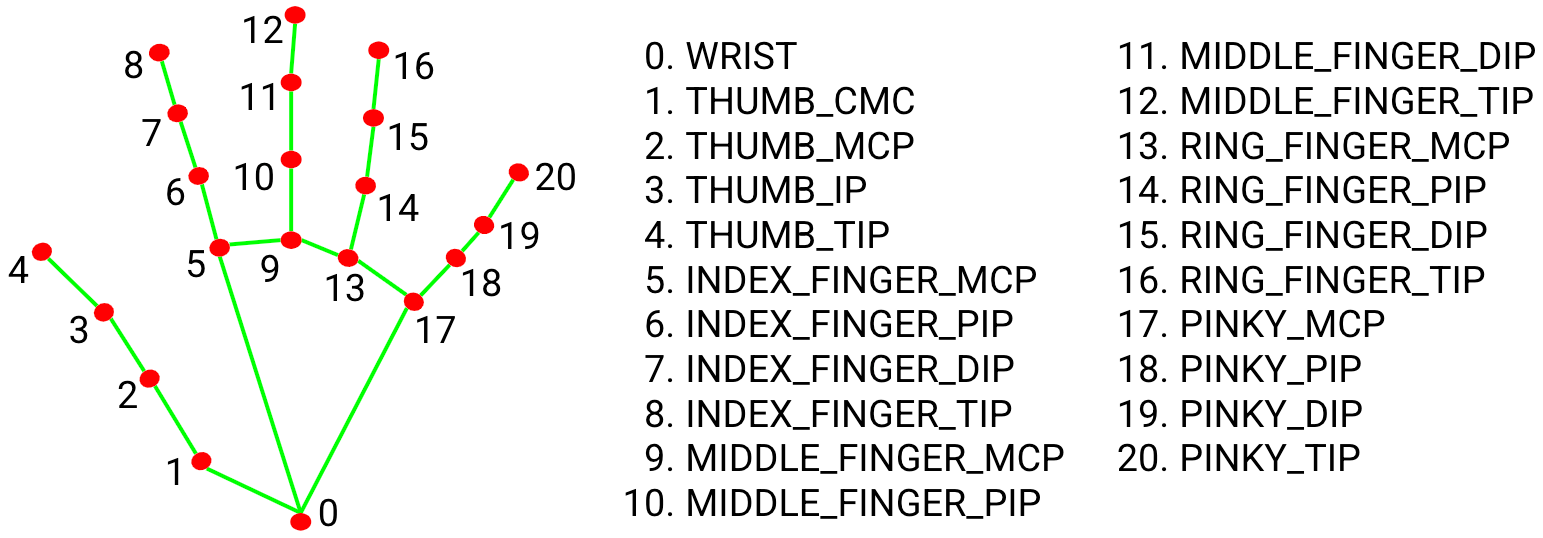
\includegraphics[width=0.95\textwidth]{MediaPipe_hands.png}
  \caption{MediaPipe Hands landmarks. Each point corresponds to a specific joint or fingertip.}
  \label{fig:mediapipe_hands}
\end{figure}

Researchers have successfully integrated MediaPipe’s tracking features into sign language 
systems to reduce the complexity of manual feature engineering. For instance, Debnath and 
Joe~\cite{ref3} demonstrate a real-time ASL detection setup where MediaPipe is employed to extract 
hand pose information, thereby reliably differentiating between common ASL hand shapes 
and movements.

\vspace{1.0em}
\noindent
\textbf{2.2.2 Depth Sensor Approaches}
\addcontentsline{toc}{subsubsection}{2.2.2 Depth Sensor Approaches}
\vspace{0.5em}

Beyond standard RGB cameras, \textit{depth sensors} capture three-dimensional information 
about hand positions. Notably, Avola et al.~\cite{ref4} illustrate how the Leap Motion Controller 
can track the skeletal structure of the hand with fine-grained accuracy, enabling precise 
measurement of joint angles. This capability is beneficial for distinguishing 
similar signs that differ only slightly in finger placement or orientation.

\vspace{1.0em}
\noindent
\textbf{2.2.3 Wearable Technology Approaches}
\addcontentsline{toc}{subsubsection}{2.2.3 Wearable Technology Approaches}
\vspace{0.5em}

Finally, some research efforts rely on \textit{wearable devices}, such as glove-based sensors, to 
record hand movements. These systems, often equipped with inertial measurement units 
(IMUs) or bend sensors, can capture motion data in three dimensions. For example, 
Stefanidis et al.~\cite{ref5} discuss the use of 3D technologies in sign language applications 
through wearable platforms. While potentially more accurate, such devices can be costly or 
cumbersome, limiting their broad adoption for everyday use.

\vspace{1.5em}
\noindent
\textbf{2.3 Summary}
\addcontentsline{toc}{subsection}{2.3 Summary}
\vspace{1em}

In summary, contemporary ASL recognition solutions range from purely vision-based 
approaches (e.g., MediaPipe Hands combined with OpenCV for live detection) to more 
specialized hardware solutions (e.g., depth sensors and wearable gloves). Among these, live 
vision-based detection using MediaPipe and OpenCV offers the optimal balance of high 
accuracy, cost-effectiveness, and ease of integration, making it the best choice for designing 
robust, real-time ASL recognition systems that can be easily adopted in real-world contexts.


%-------------------------------
%   CHAPTER 3 / Software and Application
%-------------------------------
\newpage
\section*{Chapter 3}
\addcontentsline{toc}{section}{Chapter 3}
\begin{center}
\large \textbf{Software and Application}
\end{center}

Include text here

\vspace{1.5em}
\noindent
\textbf{3.1 }
\addcontentsline{toc}{subsection}{3.1}
\vspace{1.5em}

Include text here

%-------------------------------
%   CHAPTER 4 / Results (Analysis)
%-------------------------------
\newpage
\section*{Chapter 4}
\addcontentsline{toc}{section}{Chapter 4}
\begin{center}
\large \textbf{Results}
\end{center}

Include text here

\vspace{1.5em}
\noindent
\textbf{4.1 }
\addcontentsline{toc}{subsection}{4.1}
\vspace{1.5em}

Include text here

%-------------------------------
%   CHAPTER 5 / Conclusion
%-------------------------------
\newpage
\section*{Chapter 5}
\addcontentsline{toc}{section}{Chapter 5}
\begin{center}
\large \textbf{Conclusion}
\end{center}

Include text here

\vspace{1.5em}
\noindent
\textbf{5.1 }
\addcontentsline{toc}{subsection}{5.1}
\vspace{1.5em}

Include text here

%-------------------------------
%   BIBLIOGRAPHY
%-------------------------------
\clearpage
\onehalfspacing

\renewcommand{\refname}{Bibliography}
\addcontentsline{toc}{section}{Bibliography}

\begin{thebibliography}{99}

% TerpTube
\bibitem{ref1}
E.~Hibbard \emph{et al.}, 
“Getting a Sign in Edgewise: User-Centered Design Considerations in Creating a Signed Language Mentoring Management System,” 
\emph{Sign Language Studies}, vol.~20, no.~2, pp.~264--300, 2020. 
Available: \url{https://www.jstor.org/stable/26983963}  

% Deaf info
\bibitem{ref2}
V. Falvo, L. P. Scatalon, and E. F. Barbosa, 
“The Role of Technology to Teaching and Learning Sign Languages: A Systematic Mapping,” 
in \emph{2020 IEEE Frontiers in Education Conference (FIE)}, Uppsala, Sweden, 2020, pp.~1--9, 
doi: \texttt{10.1109/FIE44824.2020.9274169}.  
Available: \url{https://ieeexplore-ieee-org.libezproxy2.syr.edu/document/9274169}

% OpenCV, MediaPipe, LSTMs 
\bibitem{ref3}
J.~Debnath and P.~J.~I R, 
“Real-Time Gesture Based Sign Language Recognition System,” 
in \emph{2024 International Conference on Advances in Data Engineering and Intelligent Computing Systems (ADICS)}, 
Chennai, India, 2024, pp.~01--06, 
doi: \texttt{10.1109/ADICS58448.2024.10533518}.
Available: \url{https://ieeexplore-ieee-org.libezproxy2.syr.edu/document/10533518}

% Leap motion sensor + LSTMs
\bibitem{ref4}
D.~Avola, M.~Bernardi, L.~Cinque, G.~L.~Foresti, and C.~Massaroni, 
“Exploiting Recurrent Neural Networks and Leap Motion Controller for the Recognition of Sign Language and Semaphoric Hand Gestures,” 
\emph{IEEE Transactions on Multimedia}, vol.~21, no.~1, pp.~234--245, Jan.~2019, 
doi: \texttt{10.1109/TMM.2018.2856094}. 
Available: \url{https://ieeexplore.ieee.org/document/8410764}

% Gloves and different wearable technologies
\bibitem{ref5}
Stefanidis, Kiriakos, Dimitrios Konstantinidis, Thanassis Kalvourtzis,  
Kosmas Dimitropoulos, and Petros Daras.  
“3D technologies and applications in sign language.” 2020. 
Available: \url{https://www.researchgate.net/publication/340966069_3D_technologies_and_applications_in_sign_language}

\bibitem{ref6}
I.~Papastratis \emph{et al.}, 
“Artificial Intelligence Technologies for Sign Language,” 
\emph{Sensors (Basel, Switzerland)}, vol.~21, no.~17, p.~5843, Aug.~30, 2021, 
doi: \texttt{10.3390/s21175843}.   
Available: \url{https://pmc.ncbi.nlm.nih.gov/articles/PMC8434597/}

% Keras textbook
\bibitem{ref7}
A.~Gulli and S.~Pal, 
\emph{Deep Learning with Keras}. 
Packt Publishing, 2018. 
Available: \url{https://books.google.com/books?id=20EwDwAAQBAJ&printsec=frontcover&source=gbs_ge_summary_r&cad=0#v=onepage&q&f=false}


% LSTMs
\bibitem{ref8}
T.~Liu, W.~Zhou, and H.~Li, 
“Sign language recognition with long short-term memory,” 
in \emph{2016 IEEE International Conference on Image Processing (ICIP)}, 
Phoenix, AZ, USA, 2016, pp.~2871--2875, 
doi: \texttt{10.1109/ICIP.2016.7532884}.  
Available: \url{https://ieeexplore-ieee-org.libezproxy2.syr.edu/document/7532884}

% ML textbook
\bibitem{ref9}
E.~Alpaydin, 
\emph{Introduction to Machine Learning}, 
The MIT Press, 4th~ed., 2020.  
Available: \url{https://books.google.com/books?id=tZnSDwAAQBAJ&printsec=frontcover#v=onepage&q&f=false}

% original project
\bibitem{ref10}
K. Takahashi, “hand-gesture-recognition-mediapipe,” GitHub repository,  
Available: \url{https://github.com/kinivi/hand-gesture-recognition-mediapipe} (Accessed: Feb. 26, 2025)

% LSTM textbook
\bibitem{ref11}
S.~Hochreiter and J.~Schmidhuber, 
“Long Short-Term Memory,” 
in \emph{Neural Computation}, vol.~9, no.~8, pp.~1735--1780, Nov.~15, 1997, 
doi: \texttt{10.1162/neco.1997.9.8.1735}. 
Available: \url{https://ieeexplore.ieee.org/document/6795963}

% RF sensors
\bibitem{ref12}
S.~Z. Gurbuz \emph{et al.}, 
“Multi-Frequency RF Sensor Fusion for Word-Level Fluent ASL Recognition,” 
\emph{IEEE Sensors Journal}, vol.~22, no.~12, pp.~11373--11381, Jun.~15, 2022, 
doi: \texttt{10.1109/JSEN.2021.3078339}. [Online].  
Available: \url{https://ieeexplore-ieee-org.libezproxy2.syr.edu/document/9425571}

% CNNs LSTMs
\bibitem{ref13}
J.~T.~S. Ru and P. Sebastian, 
“Real-Time American Sign Language (ASL) Interpretation,” 
in \emph{2023 2nd International Conference on Vision Towards Emerging Trends in Communication and Networking Technologies (ViTECoN)}, 
Vellore, India, 2023, pp.~1--6, 
doi: \texttt{10.1109/ViTECoN58111.2023.10157157}. 
Available: \url{https://ieeexplore-ieee-org.libezproxy2.syr.edu/document/10157157}

% Leap motion sensor
\bibitem{ref14}
C.-H.~Chuan, E.~Regina, and C.~Guardino, 
“American Sign Language Recognition Using Leap Motion Sensor,” 
in \emph{2014 13th International Conference on Machine Learning and Applications}, 
Detroit, MI, USA, 2014, pp.~541–544, 
doi: \texttt{10.1109/ICMLA.2014.110}. 
Available: \url{https://ieeexplore.ieee.org/document/7033173?arnumber=7033173}

% MSL (CLSTM / LSTM / RNN) MEDIAPIPE, OPENCV *PROF REC*
\bibitem{ref15}
E.~A. Borges-Galindo \emph{et al.}, 
“Sign Language Interpreting System Using Recursive Neural Networks,” 
\emph{Applied Sciences}, vol.~14, no.~18, Art. no. 8560, Sep.~23, 2024,  
Available: \url{https://www.mdpi.com/2076-3417/14/18/8560}

% Good analyze reference
\bibitem{ref16}
M.~Soundarya, M.~Yazhini, N.~Thirumala Sree, N.~Sornamalaya, and C.~Vinitha, 
“Sign Language Recognition Using Machine Learning,” 
in \emph{2024 International Conference on Advances in Computing, Communication and Applied Informatics (ACCAI)}, 
Chennai, India, 2024, pp.~1--7, 
doi: \texttt{10.1109/ACCAI61061.2024.10602025}.
Available: \url{https://ieeexplore.ieee.org/document/10602025}

% Good representation of LSTM diagram
\bibitem{ref17}
T.~Liu, W.~Zhou, and H.~Li, 
“Sign language recognition with long short-term memory,” 
in \emph{2016 IEEE International Conference on Image Processing (ICIP)}, 
Phoenix, AZ, USA, 2016, pp.~2871--2875, 
doi: \texttt{10.1109/ICIP.2016.7532884}. 
Available: \url{https://ieeexplore-ieee-org.libezproxy2.syr.edu/document/7532884}

% RNNs and LSTMs 
\bibitem{ref18}
C.~K.~M. Lee, K.~K.~H. Ng, C.-H. Chen, H.~C.~W. Lau, S.~Y. Chung, and T. Tsoi, 
“American sign language recognition and training method with recurrent neural network,” 
\textit{Expert Systems with Applications}, vol.~167, pp.~114403, 2021,  
ISSN 0957-4174.  
Available: \url{https://doi.org/10.1016/j.eswa.2020.114403} 

% Learn LSTMs
\bibitem{ref19}
C. Olah, 
“Understanding LSTM Networks,” 
Understanding LSTM Networks, Aug. 17, 2015. [Online].  
Available: \url{https://colah.github.io/posts/2015-08-Understanding-LSTMs/}


\end{thebibliography}

\end{document}

